\documentclass[a4paper, 12pt]{article}
\usepackage[T2A,T1]{fontenc}
\usepackage[utf8]{inputenc}
\usepackage[english, ukrainian]{babel}
\usepackage{amsmath}
\usepackage{amssymb}
\usepackage{mathtools}
\usepackage{euler}
% \usepackage[dvipsnames]{xcolor}
\usepackage{xcolor}
\usepackage[margin=1.5cm]{geometry}
\usepackage{float}
\usepackage{multirow}
\usepackage{multicol}
\usepackage{url}
\usepackage[unicode=true, colorlinks=true, linktoc=all, linkcolor=blue]{hyperref}
\usepackage{cite}
\usepackage{amsthm}
\usepackage{thmtools}
\usepackage[framemethod=TikZ]{mdframed}
\usepackage[toc,page,title,titletoc]{appendix}
\usepackage{bookmark}
\usepackage[nottoc,notlot,notlof]{tocbibind}
\usepackage{minted}
% \usepackage[hang]{footmisc}
\theoremstyle{definition}
\mdfdefinestyle{mdbluebox}{%
	roundcorner = 10pt,
	linewidth=1pt,
	skipabove=12pt,
	innerbottommargin=9pt,
	skipbelow=2pt,
	nobreak=true,
	linecolor=blue,
	backgroundcolor=TealBlue!5,
}
\declaretheoremstyle[
	headfont=\sffamily\bfseries\color{MidnightBlue},
	mdframed={style=mdbluebox},
	headpunct={\\[3pt]},
	postheadspace={0pt}
]{thmbluebox}

\mdfdefinestyle{mdredbox}{%
	linewidth=0.5pt,
	skipabove=12pt,
	frametitleaboveskip=5pt,
	frametitlebelowskip=0pt,
	skipbelow=2pt,
	frametitlefont=\bfseries,
	innertopmargin=4pt,
	innerbottommargin=8pt,
	nobreak=true,
	linecolor=RawSienna,
	backgroundcolor=Salmon!5,
}
\declaretheoremstyle[
	headfont=\bfseries\color{RawSienna},
	mdframed={style=mdredbox},
	headpunct={\\[3pt]},
	postheadspace={0pt},
]{thmredbox}

\declaretheorem[style=thmbluebox,name=Теорема,numberwithin=section]{theorem}
\declaretheorem[style=thmbluebox,name=Теорема,numbered=no]{theorem*}
\declaretheorem[style=thmbluebox,name=Лема,sibling=theorem]{lemma}
\declaretheorem[style=thmbluebox,name=Лема,numbered=no]{lemma*}
\declaretheorem[style=thmbluebox,name=Твердження,sibling=theorem]{proposition}
\declaretheorem[style=thmbluebox,name=Наслідок,sibling=theorem]{corollary}
\declaretheorem[style=thmredbox,name=Приклад,sibling=theorem]{example}

\mdfdefinestyle{mdgreenbox}{%
	skipabove=8pt,
	linewidth=2pt,
	rightline=false,
	leftline=true,
	topline=false,
	bottomline=false,
	linecolor=ForestGreen,
	backgroundcolor=ForestGreen!5,
}
\declaretheoremstyle[
	headfont=\bfseries\sffamily\color{ForestGreen!70!black},
	bodyfont=\normalfont,
	spaceabove=2pt,
	spacebelow=1pt,
	mdframed={style=mdgreenbox},
	headpunct={ --- },
]{thmgreenbox}

\mdfdefinestyle{mdblackbox}{%
	skipabove=8pt,
	linewidth=3pt,
	rightline=false,
	leftline=true,
	topline=false,
	bottomline=false,
	linecolor=black,
	backgroundcolor=RedViolet!5!gray!5,
}
\declaretheoremstyle[
	headfont=\bfseries,
	bodyfont=\normalfont\small,
	spaceabove=0pt,
	spacebelow=0pt,
	mdframed={style=mdblackbox}
]{thmblackbox}

% \theoremstyle{theorem}
\declaretheorem[name=Запитання,sibling=theorem,style=thmblackbox]{ques}
\declaretheorem[name=Вправа,sibling=theorem,style=thmblackbox]{exercise}
\declaretheorem[name=Зауваження,sibling=theorem,style=thmgreenbox]{remark}
\declaretheorem[name=Припущення,sibling=theorem,style=thmblackbox]{assumption}

\theoremstyle{definition}
\newtheorem{claim}[theorem]{Твердження}
\newtheorem{definition}[theorem]{Визначення}
\newtheorem{fact}[theorem]{Факт}

\newtheorem{problem}{Задача}[section]
\newtheorem{sproblem}[problem]{Задача}
\newtheorem{dproblem}[problem]{Задача}
\renewcommand{\thesproblem}{\theproblem$^{\star}$}
\renewcommand{\thedproblem}{\theproblem$^{\dagger}$}

\makeatletter
\newenvironment{solution}[1][\solutionname]{\par
  \pushQED{\qed}%
  \normalfont \topsep6\p@\@plus6\p@\relax
  \trivlist
%<amsbook|amsproc>  \itemindent\normalparindent
  \item[\hskip\labelsep
%<amsbook|amsproc>        \scshape
%<amsart|amsthm>        \itshape
\itshape 
    #1\@addpunct{.}]\ignorespaces
}{%
  \popQED\endtrivlist\@endpefalse
}
%    \end{macrocode}
%    Default for \cn{proofname}:
%    \begin{macrocode}
\providecommand{\solutionname}{Розв'язок}

\makeatother
\renewcommand{\phi}{\varphi}
\renewcommand{\epsilon}{\varepsilon}

\newcommand{\NN}{\mathbb{N}}
\newcommand{\ZZ}{\mathbb{Z}}
\newcommand{\QQ}{\mathbb{Q}}
\newcommand{\RR}{\mathbb{R}}
\newcommand{\CC}{\mathbb{C}}

\newcommand{\la}{\mathcal{L}}
\newcommand{\ca}{\mathcal{C}}
\newcommand{\hi}{\mathcal{H}}

\newcommand{\no}[1]{\left\| #1 \right\|}
\renewcommand{\sp}[1]{\left\langle #1 \right\rangle}
% \renewcommand{\sp}[2]{\left\langle #1, #2 \right\rangle}
\renewcommand{\bar}{\overline}

\newcommand*\diff{\mathop{}\!\mathrm{d}}
\newcommand*\rfrac[2]{{}^{#1}\!/_{\!#2}}

\DeclareMathOperator{\argmin}{argmin}
\DeclareMathOperator{\epigraph}{epi}
\DeclareMathOperator{\proximal}{prox}
\DeclareMathOperator{\diagonal}{diag}
\DeclareMathOperator{\domain}{dom}
\DeclareMathOperator{\trace}{tr}

\DeclareMathOperator*{\Argmin}{argmin}
\DeclareMathOperator*{\Min}{min}
\DeclareMathOperator*{\Inf}{inf}
\DeclareMathOperator*{\Sup}{sup}
\DeclareMathOperator*{\Lim}{lim}

\DeclareMathOperator*{\Sum}{\sum}
\DeclareMathOperator*{\Int}{\int}

\renewcommand{\appendixtocname}{Додаток}
\renewcommand{\appendixpagename}{Додаток}
\renewcommand{\appendixname}{Додаток}
\makeatletter
\let\oriAlph\Alph
\let\orialph\alph
\renewcommand{\@resets@pp}{\par
  \@ppsavesec
  \stepcounter{@pps}
  \setcounter{section}{0}%
  \if@chapter@pp
    \setcounter{chapter}{0}%
    \renewcommand\@chapapp{\appendixname}%
    \renewcommand\thechapter{\@Alph\c@chapter}%
  \else
    \setcounter{subsection}{0}%
    \renewcommand\thesection{\@Alph\c@section}%
  \fi
  \if@pphyper
    \if@chapter@pp
      \renewcommand{\theHchapter}{\theH@pps.\oriAlph{chapter}}%
    \else
      \renewcommand{\theHsection}{\theH@pps.\oriAlph{section}}%
    \fi
    \def\Hy@chapapp{appendix}%
  \fi
  \restoreapp
}
\makeatother

\renewcommand\thempfootnote{\alph{mpfootnote}}
\newcommand{\todo}[1]{\footnote{\textcolor{red}{TODO}: #1}}

\newcommand{\cover}[2]{
\begin{center}
\hfill \break \bf
  М{\smallІНІСТЕРСТВО ОСВІТИ ТА НАУКИ} У{\smallКРАЇНИ} \\
  К{\smallИЇВСЬКИЙ НАЦІОНАЛЬНИЙ УНІВЕРСИТЕТ ІМЕНІ} Т{\smallАРАСА} Ш{\smallЕВЧЕНКА} \\ 
  Ф{\smallАКУЛЬТЕТ КОМП'ЮТЕРНИХ НАУК ТА КІБЕРНЕТИКИ} \\
  К{\smallАФЕДРА ОБЧИСЛЮВАЛЬНОЇ МАТЕМАТИКИ}
\end{center}

\vfill 

\begin{center}
  \LARGE \bf
  Звіт до лабораторної роботи №{#1} на тему \\ 
  \guillemotleft{#2}\guillemotright
\end{center}

\vfill 

\begin{flushright}
  \large \bf 
  Виконав студент групи ОМ-3 \\
  
  Скибицький Нікіта
\end{flushright}

\vfill 

\begin{center}
  \large \bf
  Київ --- 2019
\end{center}

\thispagestyle{empty} 
\newpage
}

\author{Скибицький Нікіта}
\date{\today}

\allowdisplaybreaks
\numberwithin{equation}{section}
\linespread{1.15}

\begin{document}

\cover{1}{Метод роя часток}

\tableofcontents

\section{Неформальний опис алгоритму}

\subsection{Власне опис}

Алгоритм працює за допомогою популяції (рою) кандидатних рішень або частинок. Кожна з них рухається у обмеженій частині простору, керуючись двома факторами. Перший --- це особиста найкраща позиція частинки під час усього попереднього пошуку. Другий --- найкраще положенням по всьому рою. Тим самим у якийсь момент виникає загальна тенденція до оптимуму і рій сходиться на оптимальному розв'язку.

\subsection{Історія винаходу методу}

Метод виник в середині 90-х років ХХ сторіччя, авторами вважають психолога Джеймса Кеннеді (eng. \textit{Kennedy}) та інженера Рассела Еберхарта (eng. \textit{Eberhart}). В подальшому численні дослідники запропонували різні модифікації цього методу.

\subsection{Сфери застосування}

Взагалі кажучи, метод можна використовувати для пошуку екстремуму будь-якої функції, яка може бути обчислена на заданій множині вхідних даних і не обов'язково задана в аналітичному вигляді.

\subsection{Можливі модифікації}

\subsubsection{Збурення рою}

Однією з можливих модифікацій, яка допомагає рою виходити з локальних екстремумів є збурення рою. Це означає, що якщо більша ($> 80\%$) частина часток рою опинилася у маленькому околі якоїсь однієї точки, то у цьому околі можна лишилити лише малу ($\approx 10\%$) частину часток, а решту заново розподілити по області пошуку, наприклад рівномірним випадковим чином. \medskip

Цьому присвячені роботи \cite{eve09, lk02, xin10, xzy02}.

\subsubsection{Багатокритеріальна оптимізація}

Метод рою часто також може бути застосований до задач багато критеріальної оптимізацї, тоді функція порівняння відображає поняття парето-оптимальності, з лексикографічним способом вирішення конфліктів. \medskip

Цьому присвячені роботи \cite{pv02, cs02, mdh17}.

\section{Формалізований опис алгоритму}

Рій частинок представляє собою множину $\left\{P_j, j = \overline{1,L}\right\}$. Кожна частинка і весь рій в цілому характеризується набором параметрів, що визначає їх стан в конкретний момент часу $k$:

\begin{itemize}
    \item $X_j^{(k)} = \left( x_{j,1}^{(k)}, x_{j, 2}^{(k)}, \ldots, x_{j, n}^{(k)} \right)$, $j = \overline{1,L}$ --- положення частинки $P_j$ в $n$-вимірному просторі.

    \item Для кожної частинки $P_j$ в кожний момент часу $k$ може бути обчислене значення цільової функції, часто її називають фітнес-функцією (або функцією пристосваності): 
	\begin{equation}
	    F_j^{(k)} = F \left( X_j^{(k)} \right) = F \left( x_{j,1}^{(k)}, x_{j, 2}^{(k)}, \ldots, x_{j, n}^{(k)} \right).
	\end{equation}

    \item $V_j^{(k)} = \left( v_{j,1}^{(k)}, v_{j,2}^{(k)}, \ldots, v_{j,n}^{(k)} \right)$, $j = \overline{1,L}$ --- швидкості частинки $P_j$ в кожному напрямку.

    \item $XL_j = \left( xl_{j,1}, xl_{j, 2}, \ldots, xl_{j, n} \right)$, $j = \overline{1,L}$ --- найкраще положення частинки $P_j$ за весь час.

    \item $XG = \left( xg_1, xg_2, \ldots, xg_n \right)$ --- найкраще положення всіх частинок за весь час.
\end{itemize}

Алгоритм представляє собою ітераційний процес з дискретним часом. \medskip

На кожній ітерації кожна частинка переміщується з попереднього положення в своє нове положення за певним законом, при цьому закон переміщення кожної частинки рою враховує своє найкраще (екстремальне положення, локальний екстремум) і найкраще положення найкращої частинки рою (глобальний екстремум). \medskip

Для ініціалізації ітераційного процесу початковий стан $X_j^{(0)}$ кожної частинки $P_j$ рою визначається рівномірно розподіленою випадковою величиною заданою на вхідній множині $D$. \medskip

Початкові швидкості руху кожної частинки також визначаються як випадкові величини рівномірно розподілені на $n$-вимірному паралелепіпеді $\Pi = [- \varepsilon, \varepsilon]^n$, де $\varepsilon$ --- деяке мале число. Допускається також і нульове значення швидкості. \medskip

На кожній ітерації (в кожній момент часу) обчислюється нова швидкість кожної частинки рою за формулою:
\begin{equation}
    V_{j,i}^{(k + 1)} = \omega \cdot V_{j,i}^{(k)} + a_1 \cdot \text{rand} \cdot \left( xl_{j,i} - x_{j,i}^{(k)} \right) + a_2 \cdot \text{rand} \cdot \left( xg_{i} - x_{j,i}^{(k)} \right),
\end{equation}
де $\omega = 1 - \varepsilon$ --- коефіцієнт інерції ($\varepsilon\approx 10^{-2}$ тут вже інше), $a_1, a_2$ --- постійні значення прискорень, $\text{rand}$ --- випадкова величина рівномірно розподілена на відрізку $[0,1]$. \medskip

Після обчислення значення швидкості обчислюється нове положення кожної частинки 
\begin{equation}
    X_j^{(k + 1)} = X_j^{(k)} + V_j^{(k)}.
\end{equation}

Критерієм зупинки може бути досягнення заданого числа ітерацій або будь-який інший критерій. 

Окремо зауважимо, що якщо якась частинка $P_j$ рою виходить за межі допустимої області $D$ то її можна і варто повернути, наприклад у положення $XL_j$.

\section{Код програмного продукту}

\subsection{Використані бібліотеки}

\inputminted[firstline=2,lastline=6]{python}{../code/pso.py}

\subsection{Параметри алгоритму}

\inputminted[firstline=53,lastline=70]{python}{../code/pso.py}

\subsection{Початковий стан рою}

\inputminted[firstline=75,lastline=78]{python}{../code/pso.py}

\subsection{Побудова графіків у \texorpdfstring{$\RR^2$}{R2}}

\inputminted[firstline=83,lastline=116]{python}{../code/pso.py}

\subsection{Логування значень цільової функції}

\inputminted[firstline=121,lastline=142]{python}{../code/pso.py}

\subsection{Власне алгоритм}

\inputminted[firstline=147,lastline=167]{python}{../code/pso.py}

\section{Тестування програмного продукту}

Було розглянути три класичні тестові функції для задач оптимізації, у тому числі оптимізації з обмеженнями.

\subsection{Функція Растрігіна}

Аналітичний вигляд:

\begin{equation}
    f(x_1, \ldots, x_n) = 10 n + \Sum_{i = 1}^n x_i^2 - 10 \cos(2 \pi x_i).
\end{equation}

У коді задається наступним чином:

\inputminted[firstline=13,lastline=16]{python}{../code/pso.py}

При тестуванні на $\RR^2$ з розміром рою у $50$ часток було отримано наступний графік похибки від часу:
\begin{figure}[H]
    \centering
    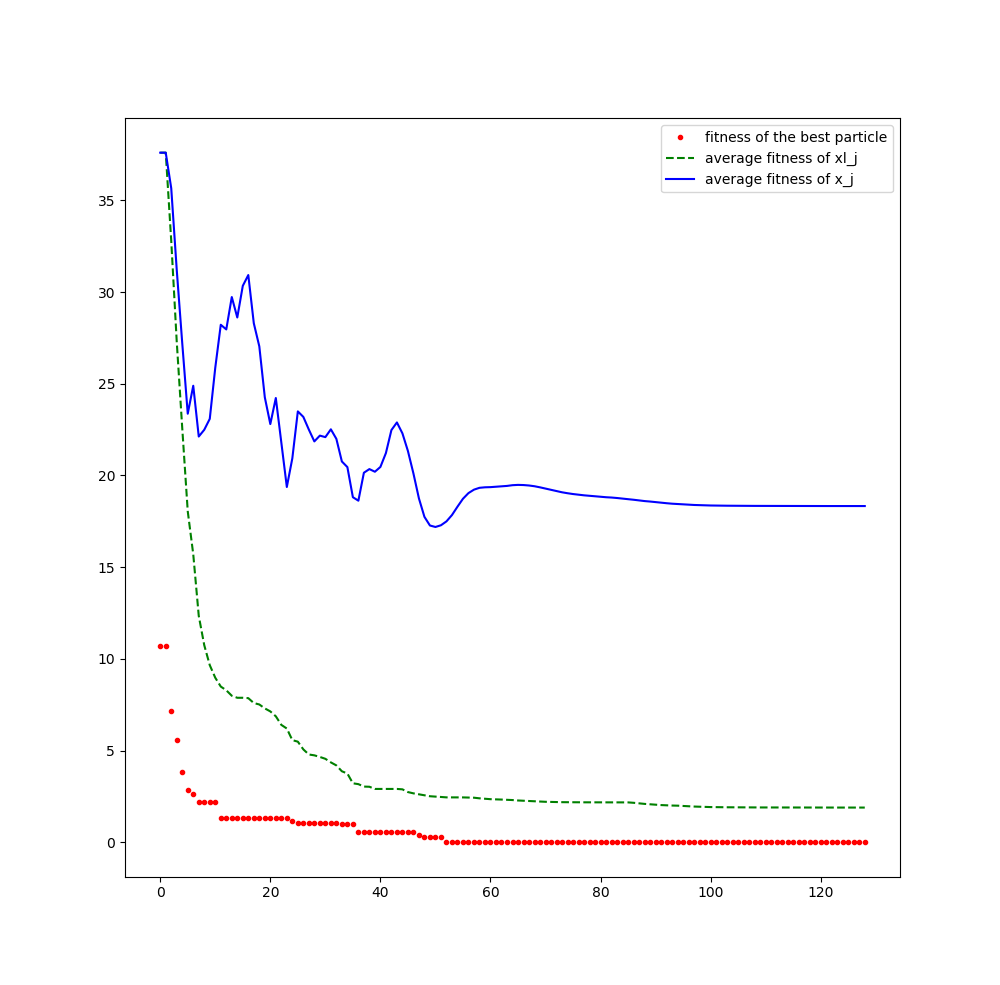
\includegraphics[width=.78\textwidth]{../code/err.png}
\end{figure}

\subsection{Функція Розенброка}

Аналітичний вигляд:

\begin{equation}
    f(x_1, \ldots, x_n) = 100 \Sum_{i = 1}^{n - 1} (x_{i + 1} - x_i)^2 + (1 - x_i)^2.
\end{equation}

У коді задається наступним чином:

\inputminted[firstline=22,lastline=25]{python}{../code/pso.py}

\subsection{Функція Розенброка з обмеженнями}

Аналітичний вигляд:

\begin{equation}
    L(x_1, \ldots, x_n) = f(x) + 100  ((x_i - 1)^3 - x_i + 1)_+^2 + 100  (x_i + x_{i + 1}^3 - 2)_+^2,
\end{equation}

де $(\cdot)_+ = \max\{ \cdot, 0\}$ --- невідє'мна частина числа. \medskip


У коді задається наступним чином:

\inputminted[firstline=31,lastline=36]{python}{../code/pso.py}

\newpage
\bibliography{main}
\bibliographystyle{ieeetr}

\end{document}